\PassOptionsToPackage{svgnames}{xcolor}
\documentclass[12pt]{article}



\usepackage[margin=1in]{geometry}  
\usepackage{graphicx}             
\usepackage{amsmath}              
\usepackage{amsfonts}              
\usepackage{framed}               
\usepackage{amssymb}
\usepackage{array}
\usepackage{amsthm}
\usepackage{multirow}
\usepackage[nottoc]{tocbibind}
\usepackage{bm}
\usepackage{enumitem}
\usepackage{tikz}
\usepackage{pdfpages}
\newcolumntype{C}[1]{>{\centering\let\newline\\\arraybackslash\hspace{0pt}}m{#1}}


  \newcommand\norm[1]{\left\lVert#1\right\rVert}
\setlength{\parindent}{0cm}
\setlength{\parskip}{0em}
\newcommand{\Lim}[1]{\raisebox{0.5ex}{\scalebox{0.8}{$\displaystyle \lim_{#1}\;$}}}
\newtheorem{definition}{Definition}[section]
\newtheorem{theorem}{Theorem}[section]
\newtheorem{notation}{Notation}[section]
\theoremstyle{definition}
\DeclareMathOperator{\arcsec}{arcsec}
\DeclareMathOperator{\arccot}{arccot}
\DeclareMathOperator{\arccsc}{arccsc}
\DeclareMathOperator{\spn}{Span}
\setcounter{tocdepth}{1}
\begin{document}

\title{Revision notes - CS2106}
\author{Ma Hongqiang}
\maketitle
\tableofcontents

\clearpage
%\twocolumn
\section{Introduction to OS}
\subsection{Operating System Basic Concepts}
\begin{definition}[Operating System]
\hfill\\\normalfont An \textbf{operating system}(OS) is a program that acts as an intermediary between a \textbf{computer user} and the \textbf{computer hardware}.
\end{definition}
The evolution of OS is as below
\[
\text{No OS}\to\text{Batch OS}\to\text{Time-sharing OS}\to\text{Personal OS}
\]
\begin{definition}[No OS]
\hfill\\\normalfont There is no OS for the first computer where programmes \textit{directly} interact with hardware, and reprogramming is done through changing the \textbf{physical configuration} of the hardware.\\
\begin{figure}[h]
\centering
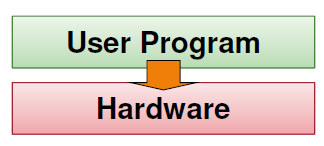
\includegraphics[width = 0.4\textwidth]{1_1.png}
\end{figure}
\textbf{Advantage}:
\begin{itemize}
  \item Minimal overhead
\end{itemize}
\textbf{Disadvantage}:
\begin{itemize}
  \item Programmes are not portable
  \item Utilisation of Computing resource is low
\end{itemize}
\end{definition}
\begin{definition}[Batch OS]
\hfill\\\normalfont Batch OS breaks down the workflow to Input, Compute and Output, which allows pipelining to occur.\\
Programmes can be \textit{submitted in batch} to be \textit{executed one at a time}. \\
\begin{figure}[h]
\centering
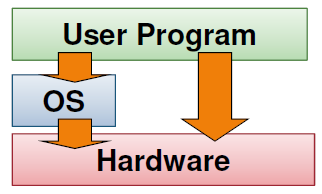
\includegraphics[width = 0.4\textwidth]{1_2.png}
\end{figure}
However, batch processing is still inefficient since the CPU will be idle when I/O. One solution is \textbf{multiprogramming}, where multiple jobs are loaded and other jobs are to be ran when I/O needs to be done.
\end{definition}
\begin{definition}[Time-sharing OS]
\hfill\\\normalfont Time-sharing OS allows multiple users to interact with machine using terminals(\textbf{teletypes}). It provides user job scheduling which gives \textit{illusion} of concurrency. \\
\begin{figure}[h]
\centering
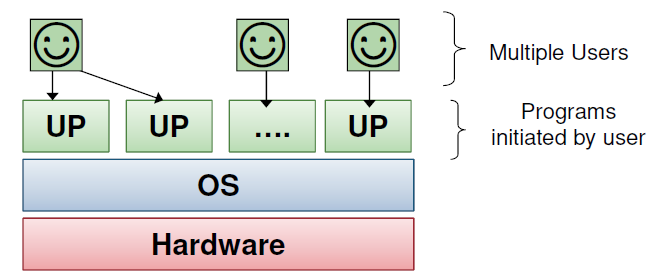
\includegraphics[width = 0.6\textwidth]{1_3.png}
\end{figure}
It provides CPU time, memory and storage management; essentially, it provides \textbf{virtualisation of hardware}, where each program executes as if it has all the resources to itself.
\end{definition}
\begin{definition}[Personal OS]
\hfill\\\normalfont Personal OS is dedicated to machine that dedicates to one user, which is not time shared.\\
There are several models:
\begin{enumerate}
  \item Windows Model:
  \begin{itemize}
    \item Single user at a time but possibly more than 1 user can access
    \item dedicated machine
  \end{itemize}
  \item Unix Model:
  \begin{itemize}
    \item One user at the workstation but others can access remotely
    \item General time sharing model
  \end{itemize}
\end{enumerate}
\end{definition}
\subsection{Motivation of OS}
There are three main motivations:
\begin{enumerate}
  \item Abstraction over the hardware, which has
  \begin{itemize}
    \item \textit{Different} capacity
    \item \textit{Different} capability, but
    \item Well-defined and \textit{common} functionality
  \end{itemize}
  so that low level details can be hidden and only high level functionality is presented. It provides efficiency and portability.
  \item Resource Allocator, which 
  \begin{itemize}
    \item Manages all resources such as CPU, Memory, I/O devices
    \item Arbitrate potentially conflicting requests, for efficient and fair resource use
  \end{itemize}
  \item Control Program, which controls execution of programmes so as to 
  \begin{itemize}
    \item Prevent errors and improper use of the computer, accidentally or maliciously
    \item Provide security and protection
  \end{itemize}
\end{enumerate}
\subsection{OS Structure}
Operating System structure needs to impart flexibility, robustness and maintainability. Generally, the high level view of OS is that
\begin{itemize}
  \item Operating system is essentially a \textbf{software}, which has the privilege to run in \textbf{kernel mode}, i.e., has complete access to all hardware resources
  \item Other software executes only in \textbf{user mode}, with limited access to hardware resources
\end{itemize}
\begin{figure}[h]
\centering
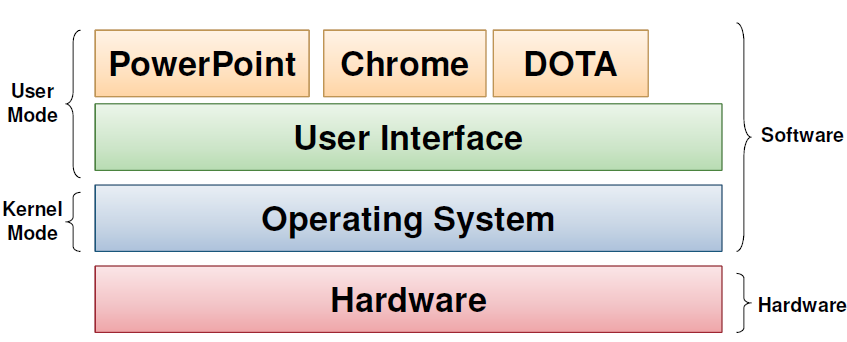
\includegraphics[width = 0.6\textwidth]{1_4.png}
\end{figure}
However, one must realise the user programme can interact with hardware through OS or else. Following diagram gives you an overview:
\begin{figure}[h]
\centering
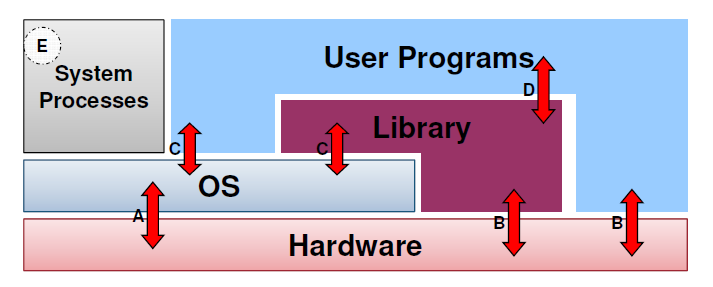
\includegraphics[width = 0.6\textwidth]{1_5.png}
\end{figure}
\begin{itemize}
  \item $A$: OS executing machine instructions
  \item $B$: normal machine instructions executed
  \item $C$: calling OS using \textbf{system call interface}, e.g. \texttt{fopen()}
  \item $D$: user program calls library code, e.g. \texttt{pow()}
  \item $E$: system processes, which provide \textit{high} level services, and is usually part of the OS
\end{itemize}

In terms of functionality, OS is known as the \textbf{kernel}, which is a programme providing special features like:
\begin{itemize}
  \item Deals with hardware issues
  \item Provides system call interface
  \item Special code for interrupt handlers, device drivers
\end{itemize}
However, kernel code has to be different than normal program as
\begin{itemize}
  \item No use of system call in kernel code
  \item Cannot use normal libraries
  \item There is no normal I/O
\end{itemize}
Currently, the common code organisation consists of
\begin{itemize}
  \item Machine independent high level language(HLL)
  \item Machine dependent HLL
  \item Machine dependent assembly code
\end{itemize}
In terms of implementation, there are few ways to structure an OS, most notably monolithic or microkernel.
\begin{definition}[Monolithic OS]
\hfill\\\normalfont Monolithic OS kernel has the defining characteristics of
\begin{itemize}
  \item One \textbf{big} special program, where various services and compopnents are integral part.
\end{itemize}
\begin{figure}[h]
\centering
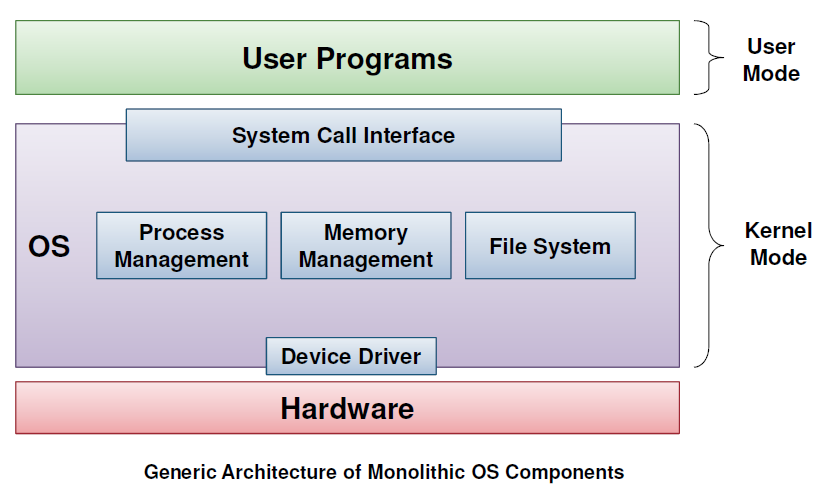
\includegraphics[width = 0.6\textwidth]{1_6.png}
\end{figure}
Monolithic kernel has the advantage of
\begin{itemize}
  \item Well understood
  \item Good performance
\end{itemize}
It has the disadvantage of
\begin{itemize}
  \item Highly coupled components
  \item Usually devolved into very complicated internal structure
\end{itemize}
\end{definition}
\begin{definition}[Microkernel OS]
\hfill\\\normalfont Microkernel OS kernel has the defining characteristics of 
\begin{itemize}
  \item Very small and clean
  \item Only provides basic and essential facilities:
  \begin{itemize}
    \item Inter-Process Communication(IPC)
    \item Address space management
    \item Thread management
    \item etc
  \end{itemize}
\end{itemize}
Higher level services like Process Management are
\begin{itemize}
  \item Built \textit{on top of} the basic facilities
  \item Run as server process \textbf{outside} of the OS
  \item Use IPC to communicate
\end{itemize}
\begin{figure}[h]
\centering
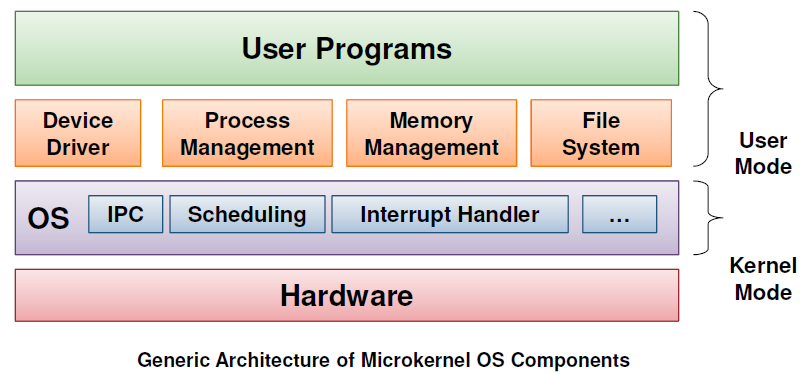
\includegraphics[width = 0.6\textwidth]{1_7.png}
\end{figure}
Microkernel OS has the advantage of
\begin{itemize}
  \item Kernel is generally more robust and more extendible
  \item Better isolation and protection between kernel and high level services
\end{itemize}
It has the disadvantage of
\begin{itemize}
  \item Lower performance
\end{itemize}
\end{definition}
Other OS structure include layered systems, client-server model etc.
\begin{definition}[Virtual Machine]
\hfill\\\normalfont Virtual Machine, or \textbf{hypervisor} is a software emulation(virtualisation) of hardware.
\end{definition}
Normal(primitive) operating systems can then run on top of the virtual machine.\\
There are two type of hypervisor:
\begin{figure}[h]
\centering
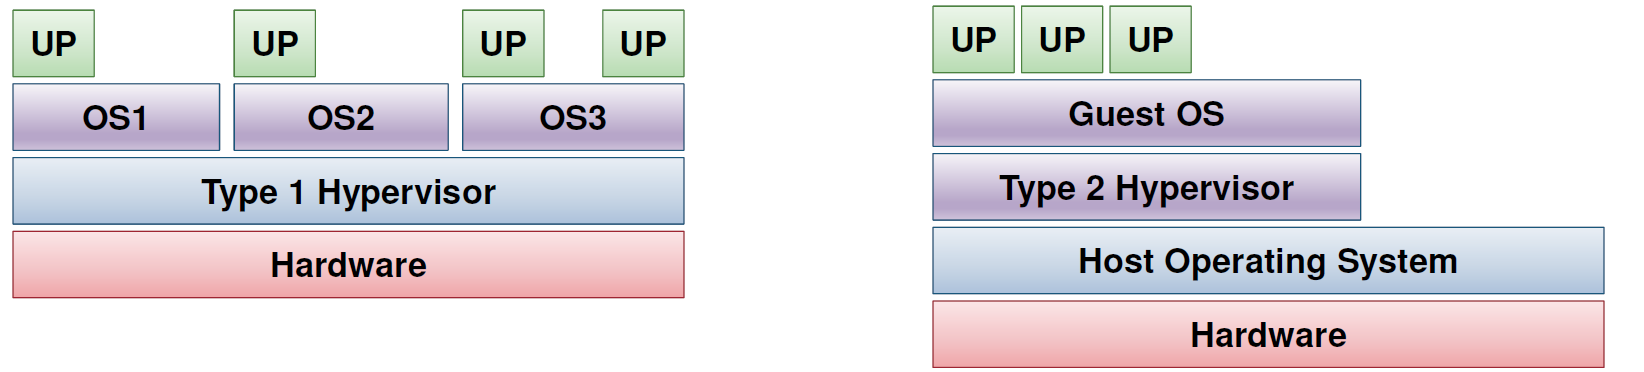
\includegraphics[width = 0.7\textwidth]{1_8.png}
\caption{Type 1 Hypervisor(left) and Type 2 Hypervisor(right)}
\end{figure}
\begin{itemize}
  \item Type 1: provides individual virtual machines to guest OSes
  \item Type 2: runs in host OS and only guest OS runs in Virtual Machine
\end{itemize}
\end{document}